\section{Implementations}

In this section, we describe our implementations of multiple heuristics, which can be found \href{https://github.com/phcentenaro7/IC-CLP/tree/main/Code/Authoral/Hummingbird}{here}.

\subsection{Wall-building}
\label{sec:wb implementation}

The wall-building (WB) heuristic attempts to load a single container by stacking cuboids within layers. A layer is a space with the same width and height as the container, but a lesser depth. To determine the depth of a layer, a box type is selected according to \cref{flow:primary box selection WBH}, where, for simplicity, \emph{box} is synonymous with \emph{box type}.

\begin{figure}[h]
    \centering
    \begin{tikzpicture}[node distance=2cm]
        \node (start) [startstop] {Start};
        \node (proc1a) [process, right of=start, xshift=2cm] {Filter boxes with\\nonzero stock};
        \node (proc1b) [process, right of=proc1a, xshift=2.75cm] {Filter boxes that\\can fit remaining depth};
        \node (dec1) [decision, below of=proc1b, yshift=-0.5cm] {Box\\list\\empty?};
        \node (dec2) [decision, below of=dec1, yshift=-1.5cm, inner sep=-0.8ex, aspect=1.5] {Any\\previously loaded\\boxes?};
        \node (proc2) [process, below of=dec2, yshift=-1cm] {Filter previously\\loaded boxes};
        \node (proc3) [process, below of=start] {Filter boxes with\\max smallest dimension};
        \node (proc4) [process, below of=proc3] {Filter boxes with\\max stock};
        \node (proc5) [process, below of=proc4] {Filter boxes with\\max greatest dimension};
        \node (proc6) [process, below of=proc5] {Select any\\filtered box};
        \node (end) [startstop, below of=proc6] {End};
        \node (proc7) [process, below of=proc2] {No further loading\\is possible};

        \draw [arrow] (start) -- (proc1a);
        \draw [arrow] (proc1a) -- (proc1b);
        \draw [arrow] (proc1b) -- (dec1);
        \draw [arrow] (dec1) -- node[anchor=east] {No} (dec2);
        \draw [arrow] (dec2) -- node[anchor=east] {Yes} (proc2);
        \draw [arrow] (dec2) -| node[xshift=2.75cm,anchor=south] {No}([xshift=1.25cm]proc3.east) -- (proc3.east);
        \draw [arrow] (proc2.west) -| ([xshift=1.25cm]proc3.east) -- (proc3.east);
        \draw [arrow] (dec1.east) -| node[xshift=-0.75cm, anchor=south] {Yes} ([xshift=0.75cm]proc7.east) -- (proc7.east);
        \draw [arrow] (proc3) -- (proc4);
        \draw [arrow] (proc4) -- (proc5);
        \draw [arrow] (proc5) -- (proc6);
        \draw [arrow] (proc6) -- (end);
        \draw [arrow] (proc7.west) -| (end.south);
    \end{tikzpicture}
    \renewcommand\figurename{Flowchart}
    \caption{Primary box selection procedure}
    \label[flowchart]{flow:primary box selection WBH}
\end{figure}

Once a box type is filtered, the feasible rotation with the greatest depth is selected, and the same depth is applied to the layer, as \cref{fig:WB layer example} shows. For unconstrained boxes, any of the six cuboid rotations is feasible. However, for boxes with a fixed height, only two rotations are feasible. \cref{fig:cuboid rotations} illustrates this.

\begin{figure}[h]
    \centering
    \begin{tikzpicture}[scale=0.25, transform shape]
        \tikzcuboidset{all faces/.style={fill=green!40}}
        \pic at (0,0,0) {cuboid=5--2--9};
        \pic at (10,0,0) {cuboid=9--2--5};
        \pic at (24,0,0) {cuboid=5--9--2};
        \pic at (33,0,0) {cuboid=2--9--5};
        \pic at (40,0,0) {cuboid=2--5--9};
        \pic at (50,0,0) {cuboid=9--5--2};
        \draw[rounded corners=0.2cm, color=red, dashed] (-1,12) rectangle(61,-3);
        \draw[rounded corners=0.2cm, color=blue, dashed] (-0.5, 5) rectangle (22, -1);
        \node[scale=4,color=red,anchor=west] at (0, 13) {Variable-height rotations};
        \node[scale=4,color=blue,anchor=west] at (0, 6) {Fixed-height rotations};
    \end{tikzpicture}
    \caption{All possible box rotations}
    \label{fig:cuboid rotations}
\end{figure}

From this point on, we refer to the box type that defines a layer's depth as its \emph{primary box type}. In its initial state, a layer contains a single empty cuboid space, which we call \emph{primary space}. Because they have the same depth, primary boxes are always loaded into primary spaces.

\begin{figure}[h]
    \centering
    \begin{tikzpicture}[scale=0.5, transform shape]
        \tikzcuboidset{hidden edges/.style={dashed}, all faces/.style={fill=blue!20}, zangle=225}
        \pic at (10,0,0) {cuboid=5--5--15};
        \tikzcuboidset*{hidden edges/.style={dashed}, all faces/.style={fill=red, fill opacity=0.3}}
        \pic at (10,0,0) {cuboid=5--5--4};
        \tikzcuboidset*{hidden edges/.style={draw=none}, all faces/.style={fill=green!40}}
        \pic at (0,0,0) {cuboid=2--2--4};
        \draw[dashed] (2,0,-3.675) -- (10,0,-3.675);
        \draw[dashed] (2,0,0) -- (10,0,0);
    \end{tikzpicture}
    \caption{A selected box (left) defining the depth of a container layer (right)}
    \label{fig:WB layer example}
\end{figure}

After the initial loading process, the primary space is divided into smaller cuboid spaces, which we call \emph{secondary spaces}. \cref{fig:remaining spaces first filling WBH A} illustrates this situation. In this example, two \emph{heightwise} spaces are created above the primary boxes, and one \emph{widthwise} space is created to their right. \cref{fig:remaining spaces first filling WBH B} shows the state of the layer after loading boxes into the widthwise space. In this case, one heightwise space is created on top of the secondary boxes, and one \emph{depthwise} space is created in front of them. The loading process is complete when none of the remaining spaces can be filled with the available box types. \cref{flow:secondary box selection WBH} is used to determine the box type for filling secondary spaces.

\begin{figure}[h]
    \centering
    \begin{subfigure}{.45\textwidth}
        \centering
        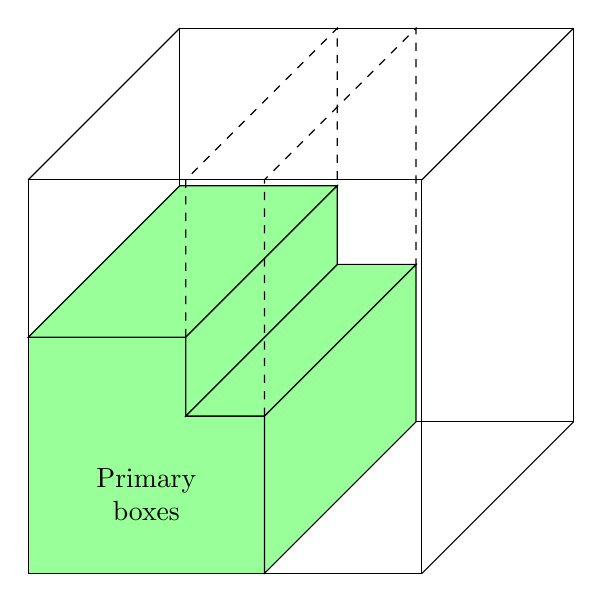
\begin{tikzpicture}[scale=0.5]
            \begin{scope}[fill=green!40]
                \draw (0,0,0) rectangle (10,10,0);
                \draw (0,0,-10) rectangle (10,10,-10);
                \draw (10,0,0) -- (10,0,-10);
                \draw (10,10,0) -- (10,10,-10);
                \draw (0,10,0) -- (0,10,-10);
                \filldraw (0,6,0) -- (0,6,-10) -- (4,6,-10) -- (4,6,0) -- cycle;
                \filldraw (0,0,0) -- (6,0,0) -- (6,4,0) -- (4,4,0) -- (4,6,0) -- (0,6,0) -- cycle;
                \filldraw (6,0,0) -- (6,0,-10) -- (6,4,-10) -- (6,4,0) -- cycle;
                \filldraw (6,4,0) -- (6,4,-10) -- (4,4,-10) -- (4,4,0) -- cycle;
                \filldraw (4,4,-10) -- (4,6,-10) -- (4,6,0) -- (4,4,0) -- cycle;
                \draw[dashed] (4,6,0) -- (4,10,0) -- (4,10,-10) -- (4,6,-10);
                \draw[dashed] (6,4,0) -- (6,10,0) -- (6,10,-10) -- (6,4,-10);
                \node[align=center] at (3,2) {Primary\\boxes};
            \end{scope}
        \end{tikzpicture}
        \caption{}
        \label{fig:remaining spaces first filling WBH A}
    \end{subfigure}
    \begin{subfigure}{.45\textwidth}
        \centering
        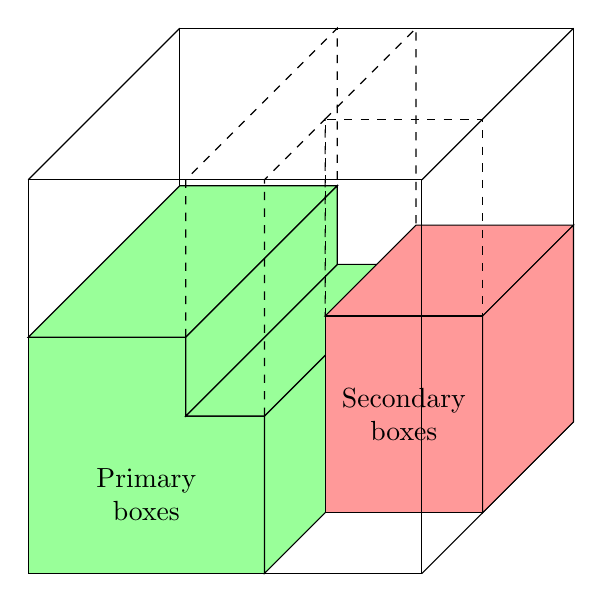
\begin{tikzpicture}[scale=0.5]
            \begin{scope}[fill=green!40]
                \draw (0,0,0) rectangle (10,10,0);
                \draw (0,0,-10) rectangle (10,10,-10);
                \draw (10,0,0) -- (10,0,-10);
                \draw (10,10,0) -- (10,10,-10);
                \draw (0,10,0) -- (0,10,-10);
                \filldraw (0,6,0) -- (0,6,-10) -- (4,6,-10) -- (4,6,0) -- cycle;
                \filldraw (0,0,0) -- (6,0,0) -- (6,4,0) -- (4,4,0) -- (4,6,0) -- (0,6,0) -- cycle;
                \filldraw (6,0,0) -- (6,0,-10) -- (6,4,-10) -- (6,4,0) -- cycle;
                \filldraw (6,4,0) -- (6,4,-10) -- (4,4,-10) -- (4,4,0) -- cycle;
                \filldraw (4,4,-10) -- (4,6,-10) -- (4,6,0) -- (4,4,0) -- cycle;
                \node[align=center] at (3,2) {Primary\\boxes};
            \end{scope}
            \begin{scope}[fill=red!40]
                \filldraw (6,5,-4) -- (6,5,-10) -- (10,5,-10) -- (10,5,-4) -- cycle;
                \filldraw (10,0,-4) -- (10,0,-10) -- (10,5,-10) -- (10,5,-4) -- cycle;
                \filldraw (6,0,-4) -- (10,0,-4) -- (10,5,-4) -- (6,5,-4) -- cycle;
                \draw (10,0,0) -- (10,10,0);
                \draw[dashed] (6,5,-4) -- (6,10,-4) -- (10,10,-4) -- (10,5,-4);
                \draw[dashed] (6,10,-4) -- (6,10,-10) -- (6,5,-10);
                \draw[dashed] (6,4,0) -- (6,10,0) -- (6,10,-4) -- (6,5,-4);
                \draw[dashed] (4,6,0) -- (4,10,0) -- (4,10,-10) -- (4,6,-10);
                \node[align=center] at (8,2.5,-4) {Secondary\\boxes};
            \end{scope}
        \end{tikzpicture}
        \caption{}
        \label{fig:remaining spaces first filling WBH B}
    \end{subfigure}
    \caption{Remaining spaces in the first filling of a layer}
    \label{fig:remaining spaces first filling WBH}
\end{figure}

\begin{figure}
    \centering
    \begin{tikzpicture}[node distance=2cm]
        \node (start) [startstop] {Start};
        \node (filter nonzero) [process,below of=start] {Filter boxes with\\nonzero stock};
        \node (generate rotation list) [process, below of=filter nonzero, yshift=-0.5cm] {Generate list\\of feasible box\\rotations};
        \node (filter fitting) [process, below of=generate rotation list, yshift=-0.5cm] {Filter rotations\\that fit in space};
        \node (check list empty) [decision, right of=filter fitting, xshift=3cm] {Box\\list\\empty?};
        \node (check multicolumn) [decision,above of=check list empty, aspect=1.5, inner sep=-1.5ex, yshift=1.5cm] {Any stock\\enough for multiple\\columns?};
        \node (select greatest area) [process, anchor=base, yshift=0.1cm] at (check multicolumn |- start.south) {Select rotation with\\greatest base area};
        \node (select greatest depth) [process, right of=check multicolumn, xshift=3cm] {Select rotation\\with greatest\\depth};
        \node (filter multicolumn) [process, below of=select greatest depth, yshift=-1.5cm] {Filter rotations\\with stock for\\multiple columns};
        \node (end) [startstop, anchor=base, yshift=-0.1cm] at (filter multicolumn |- select greatest area) {End};

        \draw [arrow] (start) -- (filter nonzero);
        \draw [arrow] (filter nonzero) -- (generate rotation list);
        \draw [arrow] (generate rotation list) -- (filter fitting);
        \draw [arrow] (filter fitting) -- (check list empty);
        \draw [arrow] (check list empty) -- node [anchor=east,yshift=-0.25cm] {No} (check multicolumn);
        \draw [arrow] (check multicolumn) -- node[anchor=east,yshift=-0.5cm] {No} (select greatest area);
        \draw [arrow] (select greatest area) -- (end);
        \draw [arrow] (filter multicolumn) -- (select greatest depth);
        \draw [arrow] (select greatest depth) -- (end);
        \draw [arrow] (check list empty.south) -| node[anchor=east, yshift=-0.25cm] {Yes} ([yshift=-0.5cm]check list empty.south) -| ([xshift=0.5cm]end.east) |- (end.east);
        \draw [arrow] (check multicolumn.east) -| node[anchor=south, xshift=-0.5cm] {Yes} ([xshift=-0.5cm]filter multicolumn.west) |- (filter multicolumn.west); 
    \end{tikzpicture}
    \renewcommand\figurename{Flowchart}
    \caption{Secondary box selection procedure}
    \label[flowchart]{flow:secondary box selection WBH}
\end{figure}

Before we discuss the loading procedure, we must introduce the concept of amalgamation. Suppose that after the layer in \cref{fig:remaining spaces first filling WBH} is fully loaded, the depthwise space created in \cref{fig:remaining spaces first filling WBH B} remains empty because no box type could fit in it. This depthwise space will be adjacent to the next layer in the container, which means it can be amalgamated with the next layer in an attempt to reduce wasted space. For instance, consider \cref{fig:amalgamation example}, which consists of the top view of two layers. The previous layer contains two empty depthwise spaces, which we assume to be at the same height or below the current layer (otherwise, no amalgamation is possible). Since space $\Omega$ has the least depth, any box we place within it is guaranteed not to overlap with other boxes from the previous layer, and thus we choose $\Omega$ to amalgamate with. After the amalgamation, the original space is split into two, $S_{L} = L$ and $S_{R} = R \cup \Omega$, with widths $w_L$ and $w_R$, respectively. However, changing these widths during loading might lead to better space utilization, which is why we introduce a \emph{flexible width} parameter, $\hat{w} = \phi w_{R}$, with $\phi \in [0,1]$. As we clarify further ahead (\cref{flow:box loading procedure WBH}), this parameter allows for the width of $S_L$ to grow to at most $w_L + \hat{w}$, with the width of $S_R$ decreasing accordingly.

\begin{figure}
    \centering
    \begin{tikzpicture}
        \fill[dashed,pattern=north east lines, pattern color=green!80] (0,0) rectangle (9,2);
        \fill[dashed,pattern=north east lines, pattern color=pink!200] (3,2) rectangle (9,3);
        \filldraw[fill=blue!40] (0,2) -- (3,2) -- (3,3) -- (5,3) -- (5,3.5) -- (9,3.5) -- (9,5) -- (0,5) -- cycle;
        \draw[{|Stealth[length=2mm]}-{Stealth[length=2mm]|}] (-0.3,2) -- (-0.3,5);
        \draw[{|Stealth[length=2mm]}-{Stealth[length=2mm]|}] (-0.3,0) -- (-0.3,2);
        \node[anchor=east, align=center] at (-0.3,3.5) {Previous\\layer};
        \node[anchor=east, align=center] at (-0.3,1) {Current\\layer};
        \draw (0,0) rectangle (9,5);
        \draw [dashed] (3,0) -- (3,2);
        \draw [dashed] (3,2) -- (9,2);
        \draw [dashed] (5,3) -- (9,3);
        \node at (6,2.5) {\huge$\Omega$};
        \node at (1.5,1) {\huge L};
        \node at (6,1) {\huge R};
    \end{tikzpicture}
    \caption{Amalgamation procedure}
    \label{fig:amalgamation example}
\end{figure}

We now describe the loading procedure. Let $B_{wh}$ be the box selected through \cref{flow:primary box selection WBH} or \cref{flow:secondary box selection WBH}, and $B_{hw}$ a rotation that swaps its width and height. If $B_{wh}$ has a fixed height, or if $B_{hw}$ does not fit in the space, then we keep $B_{wh}$. Otherwise, if enough stock exists to complete a column with either rotation, we select the rotation that results in the highest column. If neither rotation completes a column, we choose the rotation with the greatest height. This leads us to \cref{flow:box loading procedure WBH}, which describes how spaces are filled using the selected box type. Since spaces are filled by side-by-side columns of a single box rotation, determining the cuboid spaces that remain after loading is trivial.

\begin{figure}[h]
    \centering
    \begin{tikzpicture}[node distance=2cm]
        \node (start) [startstop] {Start};
        \node (check nonzero stock) [decision, below of = start, yshift=-2cm, inner sep=0.2ex] {Box\\stock\\nonzero?};
        \node (check next placement) [decision, right of = check nonzero stock, xshift=3cm] {Next box\\exceeds space\\width?};
        \node (check amalgam overlap) [decision, right of = check next placement, xshift=3cm] {Space\\overlaps with\\amalgam?};
        \node (check flexible width) [decision, below of = check amalgam overlap, yshift=-2cm, inner sep=0.2ex] {Box\\exceeds\\$w_L + \hat{w}$?};
        \node (place column) [process, above of=check next placement, yshift=1cm] {Place box column};
        \node (adjust widths) [process, left of=check flexible width, xshift=-3cm] {Adjust space and\\amalgam widths};
        \node (place column 2) [process, below of=adjust widths, yshift=0.25cm] {Place box column};
        \node (end) [startstop, left of=place column 2,xshift=-3cm, yshift=-1cm] {End};
        
        \draw [arrow] (start) -- (check nonzero stock);
        \draw [arrow] (check nonzero stock) -- node [anchor=south] {Yes} (check next placement);
        \draw [arrow] (check nonzero stock) -- node [anchor=east] {No} (end);
        \draw [arrow] (check next placement) -- node [anchor=east] {No} (place column);
        \draw [arrow] (check next placement) -- node [anchor=south] {Yes} (check amalgam overlap);
        \draw [arrow] (check amalgam overlap) -- node [anchor=east] {Yes} (check flexible width);
        \draw [arrow] (check flexible width) -- node [anchor=south] {No} (adjust widths);
        \draw (place column.west) -| (check nonzero stock.north);
        \draw [arrow] (check flexible width.south) |- (end.east);
        \draw (check amalgam overlap.east) -- node [anchor=south] {No} +(0.5cm,0) |- (end.east);
        \draw [arrow] (adjust widths) -- (place column 2);
        \draw [arrow] (place column 2) |- (end.east);
        % \draw (check amalgam overlap.east) -- +(0.5cm,0) |- (check)
    \end{tikzpicture}
    \renewcommand\figurename{Flowchart}
    \caption{Box loading procedure}
    \label[flowchart]{flow:box loading procedure WBH}
\end{figure}

With this procedure, a single container can be loaded with items. To generalize the loading process to multiple containers, \cref{alg:wb mclp} is used.

\begin{algorithm}
    \begin{algorithmic}[1]
        \floatname{algorithm}{Algorithm}
        \caption{Wall-building heuristic for multiple containers}\label[algorithm]{alg:wb mclp}
        \State $C_{List} \gets \text{List of containers obtained through IP model}$
        \While{there are items left to load}
            \State apply primary box selection procedure to remaining item types
            \State $L_{depth} \gets \text{depth of the new layer}$
            \For{$C$ \textbf{in} $C_{List}$}
                \State $C_{depth} \gets \text{depth of remaining unfilled space in $C$}$
                \If{$C_{depth} \geq L_{depth}$}
                    \State apply placement procedure to $C$
                    \Break
                \EndIf
            \EndFor
            \If{placement procedure not applied}
                \State \Return cannot place all the items
            \EndIf
        \EndWhile
        \State \Return all items placed
    \end{algorithmic}
\end{algorithm}

\subsection{Genetic algorithm}

The GA developed is a simplified version of the one presented by \textcite{GONÇALVES2011}. To understand this method, we first need to enumerate the different item types from 1 to $n$. Then, let $q_1, \dots, q_n$ be the quantities of each item type. A non-decreasing sequence $S$ can be defined, containing item $k$ a total of $q_k$ times, for $k = 1,\dots,n$. For example, given 3 item types with $q_1 = q_2 = 2$, $q_3 = 1$, it follows that $S = (1, 1, 2, 2, 3)$.

For a problem with $Q = \sum_{k=1}^{n}q_k$ items, a population of chromosomes with $2Q$ genes is generated, with values in the $[0, 1]$ interval. The first $Q$ genes specify the order in which the heuristic attempts to place items. This is done by associating each gene to the item type with the same index in $S$, and then reordering $S$ the same way as needed to put the first $Q$ genes in ascending order. As an example, suppose $S = (1, 1, 2, 2, 3)$, and a chromosome whose first five genes are $(0.93, 0.42, 0.17, 0.48, 0.80)$. If we rearrange these numbers in ascending order, we obtain $(0.17, 0.42, 0.48, 0.80, 0.93)$. By equivalently swapping the items in $S$, we get its rearrangement, $\bar{S} = (2, 1, 2, 3, 1)$.

The remaining $Q$ genes inform how each item must be placed. Specifically, gene $g_{Q+k}$ is used to determine the rotation and plane of item $\bar{S}_k$, $k = 1, \dots, Q$. Valid rotations for an item can be either variable- or fixed-height rotations, as shown in \cref{fig:cuboid rotations}. The plane can be $xy$, $xz$ or $yz$, and it indicates the axes along which the item is placed. \cref{fig:xy plane example} illustrates the filling of a cuboid space along the $xy$ plane, supposing that there are four items to place. The process consists of selecting one of the axes, $x$ or $y$, and attempting to fill it with as many strips of items as possible, such that the resulting packing is a cuboid. In the first packing, the $x$ plane is prioritized. As a result, one horizontal strip with two items is placed. Since there is enough vertical and horizontal space left, another strip of two boxes is placed on top of the first. In the second packing, the $y$ plane is prioritized. Three items can be stacked vertically, which leaves one. This remaining item is not enough to complete another column, therefore it is not placed.

\begin{figure}[h]
    \centering
    \begin{tikzpicture}[scale=0.5, transform shape]
        \tikzcuboidset{hidden edges/.style={dashed}, all faces/.style={fill=blue!20}, zangle=225}
        \pic at (0,0,0) {cuboid=5--5--5};
        \draw[-stealth, ultra thick] (-2.5,0,0) -- (-1, 0, 0) node[right]{\scalebox{2}{$x$}};
        \draw[-stealth, ultra thick] (-2.5,0,0) -- (-2.5, 1.5, 0) node[above]{\scalebox{2}{$y$}};
        \draw[-stealth, ultra thick] (-2.5,0,0) -- (-2.5, 0, -3) node[above]{\scalebox{2}{$z$}};
        \tikzcuboidset*{hidden edges/.style={dashed}, all faces/.style={fill=red, fill opacity=0.3}}
        \draw[-stealth, ultra thick] (7,3.5,0) -- (9,3.5,0);
        \tikzcuboidset{hidden edges/.style={dashed}, all faces/.style={fill=blue!20}, zangle=225}
        \pic at (9.3,0,0) {cuboid=5--5--5};
        \pic at (18,0,0) {cuboid=5--5--5};
        \draw (17,3.5,0) node{\huge{or}};
        \tikzcuboidset{all faces/.style={fill=yellow!20}, zangle=225}
        \pic at (0,0,0) {cuboid=2--1.5--2.75};
        \pic at (9.3,0,0) {cuboid=2--1.5--2.75};
        \pic at (11.3,0,0) {cuboid=2--1.5--2.75};
        \pic at (9.3,1.5,0) {cuboid=2--1.5--2.75};
        \pic at (11.3,1.5,0) {cuboid=2--1.5--2.75};
        \pic at (18,0,0) {cuboid=2--1.5--2.75};
        \pic at (18,1.5,0) {cuboid=2--1.5--2.75};
        \pic at (18,3,0) {cuboid=2--1.5--2.75};
        \tikzcuboidset{all faces/.style={fill=blue!20}, zangle=225}
        \pic at (18,5,0) {cuboid=5--0--5};
        \pic at (23,0,0) {cuboid=0--5--5};
        \pic at (9.3,5,0) {cuboid=5--0--5};
        \pic at (14.3,0,0) {cuboid=0--5--5};
        \pic at (0,5,0) {cuboid=5--0--5};
        \pic at (5,0,0) {cuboid=0--5--5};
    \end{tikzpicture}
    \caption{Two possible ways of filling the $xy$ plane of a given space with a cuboid item}
    \label{fig:xy plane example}
\end{figure}

Since there are at most six rotations, and each plane can be filled in two different ways, there is a maximum of 36 possible ways to place an item in a given space. In order to select one of the item configurations, all possibilities are mapped to different subintervals of equal length of $[0,1]$. Then, whichever interval the respective gene belongs to is used to define the item's placement.

To select the space in which to place an item, the back-bottom-left procedure (BBL) is used. Let $E_k$ be the $k$-th empty space available for packing. BBL orders spaces such that $E_i < E_j$ if $x_i < x_j$, or $x_i = x_j$ and $y_i < y_j$, or $x_i = x_j$ and $y_i = y_j$ and $z_i < z_j$. Then, the first space in the ordering where the item fits is selected. After an item is placed, new empty cuboid spaces are created, adjacent to the item. To calculate these spaces, the method described by \textcite{LAI1997} is used, with one difference: The space on top of the item is limited to the area the item occupies. This is to guarantee the vertical stability of items, by ensuring that they are either placed on the ground or that their base area is completely supported by an item directly below.

In order to extend the GA by \textcite{GONÇALVES2011} to multiple containers, the BBL procedure is applied to the first container in the sequence. If the current item does not fit in any of the remaining spaces, the next container in the sequence is selected, and the BBL procedure is applied again. This process is repeated until a fitting space is found, or there are no containers left to check.

A chromosome's fitness is calculated as follows: Let $V_{Ti}$ and $V_{Fi}$ be, respectively, the total and the filled volume of container $i$. Let $k$ be the number of containers in the sequence determined by the IP model. We first calculate the fitness of a given chromosome as:

\begin{equation}
    F = \frac{100}{k}\sum_{i=1}^{k}\frac{V_{Fi}}{V_{Ti}}.
\end{equation}

Which gives us the mean percentage of filled volume per container. Now let $L$ be the number of items left out of the containers after the packing process is finished. If $L > 0$, a penalty must be applied to the fitness value. In our case, we chose

\begin{equation}
    \bar{F} = \frac{F}{10L}
\end{equation}
as the new fitness value, because it greatly decreases with the number of items that are left outside of the containers.

Once a population is generated and the fitness value of each solution is determined, the chromosomes are sorted according to their fitness values. A certain number of top solutions, called the population's elite, is immediately copied to the next population. Another set of chromosomes of the next population is randomly generated, which can be interpreted as a form of mutation. Finally, the remaining spots left in the next population are filled by chromosomes resulting from the crossover of randomly selected elite solutions and randomly selected solutions from the entirety of the population.